\documentclass{article}
\usepackage[utf8]{inputenc}
\usepackage{preamble}

\begin{document}

\begin{center}
   \LARGE{\textsc{MATH 271, Mini Project}}\\
   \large{\textsc{Due December 20$^\textrm{th}$}}
\end{center}
\vspace{.5cm}

\section*{Solving the POAR Problem}

Here we will go about solving the particle on a ring problem.  We will set up the differential equation for a free particle, and determine the set of orthonormal basis states for this system.  In doing so, we will realize that (by the linearity of Schr\"odinger's equation) a superposition of solutions can be written as infinite sums satisfying a normalization condition.  

\begin{solution}{}{prob1}
		If we want our particle to be free on the ring, what is the potential for this system?
		\tcblower
		The potential for the \boldblue{free particle} on a ring is $V(x)=0$. The potential is an external field that imposes a force on a particle by
		\[
		F(x)=-\frac{d}{dx}V(x).
		\]
		That is, the derivative of the potential is a force.  Hence, we could in fact take $V(x)=C$ for any constant $C\in \R$ and we would recover the same kinematics.
\end{solution}

\begin{solution}{}{prob2}
		What are the ``boundary" conditions we place on $\Psi(x)$? \emph{Hint: think about what happens as we consider how the function changes as we move all the way around the ring.}
		\tcblower
		The word boundary is used here in a rather incorrect way.  A ring is a geometrical shape that has no boundary! Hence, we need to make our solution $\Psi$ aware of this fact.  The function $\Psi$ must be continuous and differentiable in order to be physically reasonable. Hence, in order to force $\Psi$ to be a continuous and differentiable function on the circle we must first note that for the coordinate $x\in [0,L]$ that $x=0$ and $x=L$ are being identified as the same point around the circle. We see this in the diagram.
		
\begin{figure}[H]
	\centering 
	%\def\svgwidth{0.75\columnwidth} 
	\resizebox{.55\textwidth}{!}{\input{POAR.pdf_tex}}
\end{figure}
		
		Hence, $\Psi$ can only be continuous if $\Psi(0)=\Psi(L)$ and the function can only be differentiable everywhere if we require $\Psi'(0)=\Psi'(L)$. These will act as our boundary conditions. Sometimes these conditions are referred to as \boldblue{periodic boundary conditions}.
\end{solution}

\begin{solution}{}{prob3}
		State the full differential equation and include the boundary conditions.
		\tcblower
		With what we have above, we can now write out the whole problem. Note that we have
		\[
		H = \frac{-\hbar^2}{2m}\frac{d^2}{dx^2},
		\]
		since $V(x)=0$. Hence, we are wishing to solve the boundary value problem
		\begin{align*}
					\frac{-\hbar^2}{2m}\frac{d^2\Psi}{dx^2}(x)=E\Psi(x) \quad \textrm{on $[O,L]$}\\
					\textrm{with}~ \Psi(0)=\Psi(L) \quad \textrm{and}\quad \Psi'(0)=\Psi'(L). 
		\end{align*}
\end{solution}

\begin{solution}{}{prob4}
		What is the order and type of this differential equation.
		\tcblower
		The above equation is a second order homogeneous linear ordinary differential equation with constant coefficients.  We can see this since a second order linear equation takes the form
		\[
		u''(x)+f(x)u'(x)+g(x)u(x)=h(x).
		\]
		We can rewrite our equation in this form as
		\[
		\Psi''(x)+\frac{2mE}{\hbar^2}\Psi(x)=0.
		\]
		Let us put $\omega^2=\frac{2mE}{\hbar^2}$ so that we then have the equation
		\[
		\Psi''(x)+\omega^2\Psi(x)=0,
		\]
		which is the equation for the \boldblue{Harmonic oscillator}.
	\end{solution}

\begin{solution}{}{prob5}
		Find the general solution to the differential equation.
		\tcblower
		We have solved the harmonic oscillator equation before, but can solve it again rather quickly by noting that the characteristic polynomial for this equation is $\lambda^2+\omega^2$. We can realize this characteristic polynomial as coming from a matrix in the following way.  First, let $\vartheta(x)=\Psi'$, and hence we have two first order linear equations
		\begin{align*}
			\Psi'(x)&=\vartheta(x)\\
			\vartheta'(x)&=-\omega^2 \Psi(x).
		\end{align*}
		We can write this as a matrix equation by
		\[
		\begin{pmatrix} \Psi'(x) \\ \vartheta'(x) \end{pmatrix} = \begin{pmatrix} 0 & 1 \\ \omega^2 & 0 \end{pmatrix} \begin{pmatrix} \Psi(x) \\ \vartheta(x)\end{pmatrix}.
		\]
		In other words, letting
		\[
		\vecv=\begin{pmatrix} \Psi(x) \\ \vartheta(x) \end{pmatrix} \qquad \textrm{and} \qquad [A]=\begin{pmatrix} 0 & 1 \\ \omega^2 & 0 \end{pmatrix},
		\]
		we have the equation
		\[
		\vecv' = [A]\vecv.
		\]
		Then, we can find the eigenvalues of $[A]$ by
		\[
		\det([A]-\lambda[I])=0,
		\]
		in which we get the characteristic polynomial we stated before
		\[
		\lambda^2+\omega^2=0.
		\]
		Though we did not discuss it explicitly in class, this is where the characteristic polynomial comes from in the second order equations we solved.  There's a bit more work to be shown in why this is the correct approach, but we won't do that for now.
		
		From the characteristic equation, we have $\lambda=\pm i\omega$ which gives rise to the general solution
		\[
		\boxed{\Psi(x)=C_1 e^{i\omega x}+C_2 e^{-i\omega x}}.
		\]
	\end{solution}

\begin{solution}{}{prob6}
		Apply the boundary conditions to determine $E$. There should be an energy value for every integer $n\geq 0$.
		\tcblower
		Now, we can apply the periodic boundary conditions. First, we have
		\[
		\Psi(0)=\Psi(L)
		\]
		which gives us
		\[
		C_1+C_2 = C_1 e^{i \omega L} + C_2 e^{i\omega L}.
		\]
		Since these must equal for any choices of the unknown constants $C_1$ and $C_2$, we must have that
		\[
		\omega L = 2n\pi,
		\]
		since $e^{ix}$ is a periodic function with period $2\pi$. Now, the second boundary conditions do not add further restrictions since if we take
		\[
		\Psi'(0)=\Psi'(L),
		\]
		we get
		\[
		i\omega C_1-i\omega C_2=i\omega C_1 e^{i\omega L}-i\omega C_2 e^{-i\omega L}.
		\]
		This equation does not add any further restrictions on $\omega$.
		
		Recall that
		\[
		\omega^2 = \frac{2mE}{\hbar^2}
		\]
		and thus
		\[
		E=\frac{\omega^2\hbar^2}{2m},
		\]
		and since $\omega=\frac{2n\pi}{L}$, we have
		\[
		\boxed{E=\frac{2n^2\pi^2\hbar^2}{mL^2}}
		\]
	\end{solution}

\begin{solution}{}{prob7}
		What are the differences in the solutions between the POAR and the free particle in a 1-dimensional box?
		\tcblower
		We found that there is a general solution for every integer $n$ which is given by
		\[
		\psi_n(x) = C_1e^{i\omega x}+C_2 e^{-i\omega x},
		\]
		which we can split into an even and an odd part using Euler's formula. Specifically, this gives us
		\[
		\boxed{\psi_n^e(x) = C_n^e \cos\left(\frac{2n\pi x}{L}\right)} \qquad \textrm{and} \qquad \boxed{\psi_n^o(x) = C_n^o \sin\left(\frac{2n\pi x}{L}\right)} \qquad \textrm{for $n=0,1,2,3,\dots$}.
		\]
		Note that for $n<0$, we will have redundant states, so we need not include these values. Also, the $n=0$ state is degenerate in that the solution is actually a constant function. That is,
		\[
		\psi_0(x) = C_0,
		\]
		since $\cos(0)=1$, and $\sin(0)=0$.	Then, for the particle in the 1-dimensional box we simply had the general solutions given by
		\[
		\varphi_n(x) = C_n \sin\left(\frac{n\pi x}{L}\right) \qquad \textrm{for $n=1,2,3,\dots$},
		\]
		which are the odd states of the POAR problem. In the 1-dimensional box case, we did not have a constant function as a solution since the wave function had to be zero at the boundaries. Since the POAR problem had no boundaries, we did not have this issue. Moreover, we include the even solutions to the equation (the cosine and constant functions) which were not solutions to the boundary value problem for the 1-dimensional box.
		
		Lastly, we can see that the energies per state are slightly different. For the particle in a box, we had the energy
		\[
		E_{n,\textrm{box}} = \frac{n^2\hbar^2 \pi^2}{2mL} \qquad n=1,2,3,\dots,
		\]
		and the energies for the POAR problem are
		\[
		E_n = \frac{2n^2\hbar^2\pi^2}{mL} \qquad n=0,1,2,3,\dots,
		\]
		which are greater by a factor of four. Note that there is also a zero energy state in this case!
	\end{solution}

\begin{solution}{}{prob8}
		For a fixed $n$, show that
		\[
		\int_0^L \sin\left(\frac{2n\pi x}{L}\right)\cos\left(\frac{2n\pi x}{L}\right)dx =0,
		\]
		which shows that the sine and cosine functions above are orthogonal.
		\tcblower
		We can integrate this using Wolfram alpha by entering
		\begin{verbatim}
			Integrate[sin(2n pi x/L)\cos(2n pi x/L),{x,0,L}]
		\end{verbatim}
		which outputs
		\[
		\int_0^L \sin\left(\frac{2n\pi x}{L}\right)\cos\left(\frac{2n\pi x}{L}\right)dx = \frac{L\sin^2(2 n \pi)}{4\pi n}
		\]
		which is indeed equal to zero when $n>0$ since $\sin(2 n \pi)=0$ for any integer $n$.  Note that for the case when $n=0$, we have that $\sin(0)=0$ and $\cos(0)=1$, and hence we also have the above integral is zero when $n=0$. Thus the even and odd states of the POAR are orthogonal to each other for every $n$.
	\end{solution}

\begin{solution}{}{prob9}
		Determine the normalization constant $C$ for each state. Note that this constant is the same for each state except for the state corresponding to $n=0$ (so you must find that one as well). Can you argue why this is the case?
		\tcblower
		Note that the functions $\cos^2\left(\frac{2n\pi x}{L}\right)$ and $\sin^2\left(\frac{2n\pi x}{L}\right)$ oscillate sinusoidally at the same rate with a period of $\frac{L}{2}$ and same magnitude and thus will have the integral value.  So, for the $n>0$ case, it suffices to compute
		\[
		1=\int_0^L \left| C\psi_n^e(x)\right|^2 dx = \int_0^L |C|^2 \cos^2\left(\frac{2n\pi x}{L}\right) dx  = \frac{L (4\pi n+\sin(4\pi n))}{8\pi n}.
		\]
		Then note that for $n$ an integer greater than zero, we have
		\[
		1 = |C_n|^2 \frac{L}{2},
		\]
		which gives us that
		\[
		\boxed{C_n= \sqrt{\frac{2}{L}}.}
		\]
		Note that this $C_n$ does not depend on $n$ either. This gives us the normalized states
		\[
		\boxed{\psi_n^e(x) = \sqrt{\frac{2}{L}} \cos\left(\frac{2n\pi x}{L}\right)} \qquad \textrm{and} \qquad \boxed{\psi_n^o(x) = \sqrt{\frac{2}{L}} \sin\left(\frac{2n\pi x}{L}\right)} \qquad \textrm{for $n=1,2,3,\dots$}.
		\]
		
		In the case where $n=0$, our solution function was constant, so we must find
		\[
		1=\int_0^L |C_0|^2 dx = |C_0|^2 L,
		\]
		and so when $n=0$ we have the state
		\[
		\boxed{\psi_0(x)=\sqrt{\frac{1}{L}}.}
		\]
	\end{solution}

\begin{solution}{}{prob10}
		Use orthogonality to show that the above statement is true.
		\tcblower
		Consider
		\[
		\langle \Psi(x),\psi_n^e(x)\rangle = \int_0^L \Psi(x)\psi_n^{e^*}(x)dx.
		\]
		We can write this out
		\begin{align*}
			 \int_0^L \Psi(x)\psi_n^{e^*}(x)dx &= \int_0^L \left(a_0 \psi_0(x) + \sum_{n=1}^\infty a_n^e \psi_n^e(x) + \sum_{n=1}^\infty a_n^o \psi_n^o(x)\right) \psi_n^{e^*}(x)dx\\
			 &= a_n^e\int_0^L \psi_n^e(x)\psi_n^{e^*}(x)dx\\
			 &= a_n^e.
		\end{align*}
		Note that in the above we used orthogonality of the states as well as the fact that they are normalized. The result is analogous for the other states $\psi_n^o(x)$ and $\psi_0(x)$.
	\end{solution}

\begin{solution}{}{prob11}
	Show that the $\Psi(x)$ written as a superposition above is a normalized solution to the POAR problem.
	\tcblower
	First, note that the ODE for the POAR problem is linear and hence a superposition of solutions is also a solution. So, it must be that $\Psi(x)$ is a solution.
	
	Now, to see that $\Psi(x)$ is normalized, we must show that
	\[
	\int_0^L |\Psi(x)|^2dx = 1,
	\]
	or equivalently that
	\[
	\langle \Psi(x), \Psi(x) \rangle = 1.
	\]
	Since we have normalized each state, and shown that each is mutually orthogonal, we can simplify the above inner product quite a bit.  We have
	\begin{align*}
		\langle \Psi(x),\Psi(x)\rangle &= \left\langle a_0 \psi_0 + \sum_{n=1}^\infty a_n^e \psi_n^e(x) + \sum_{n=1}^\infty a_n^o \psi_n^o(x), \Psi(x)\right\rangle\\
		&= a_0 \langle \psi_0(x),\Psi(x)\rangle +\sum_{n=1}^\infty a_n^e \langle \psi_n^e(x),\Psi(x)\rangle + \sum_{n=1}^\infty a_n^o \langle \psi_n^o(x),\Psi(x)\rangle,
	\end{align*}
	where we used the linearity of the inner product as well.  Now, note that we have
	\begin{align*}
		\langle \psi_0(x), \Psi(x)\rangle = a_0^* \qquad \langle \psi_n^e(x),\Psi(x)\rangle = a_n^{e^*} \qquad \langle \psi_n^o(x),\Psi(x)\rangle =a_n^{o^*},
	\end{align*}
	by orthogonality.  Hence, continuing the previous work, we have
	\[
	 a_0 \langle \psi_0(x),\Psi(x)\rangle +\sum_{n=1}^\infty a_n^e \langle \psi_n^e(x),\Psi(x)\rangle + \sum_{n=1}^\infty a_n^o \langle \psi_n^o(x),\Psi(x)\rangle = a_0a_0^* + \sum_{n=1}^\infty a_n^e a_n^{e^*}+\sum_{n=1}^\infty a_n^oa_n^{o^*}
	\]
	which gives us
	\[
	\langle \Psi(x),\Psi(x)\rangle = |a_0|^2 + \sum_{n=1}^\infty |a_n^e|^2 +\sum_{n=1}^\infty |a_n^o|^2 =1.
	\]
	Thus we have that $\Psi(x)$ is normalized.
	\end{solution}

\begin{solution}{}{prob12}
		Plot this function only on the region $[0,L]$ using Desmos.
		\tcblower
		We can input
		\begin{verbatim}
		{x<L/2:0,x>=L/2:1}{0<=x<=L}
		\end{verbatim}
		into Desmos which will allow us to add a slider for $L$. This will plot $f(x)$ only on the desired region (a chosen $L$). Here we have it plotted.
		\begin{figure}[H]
			\centering
			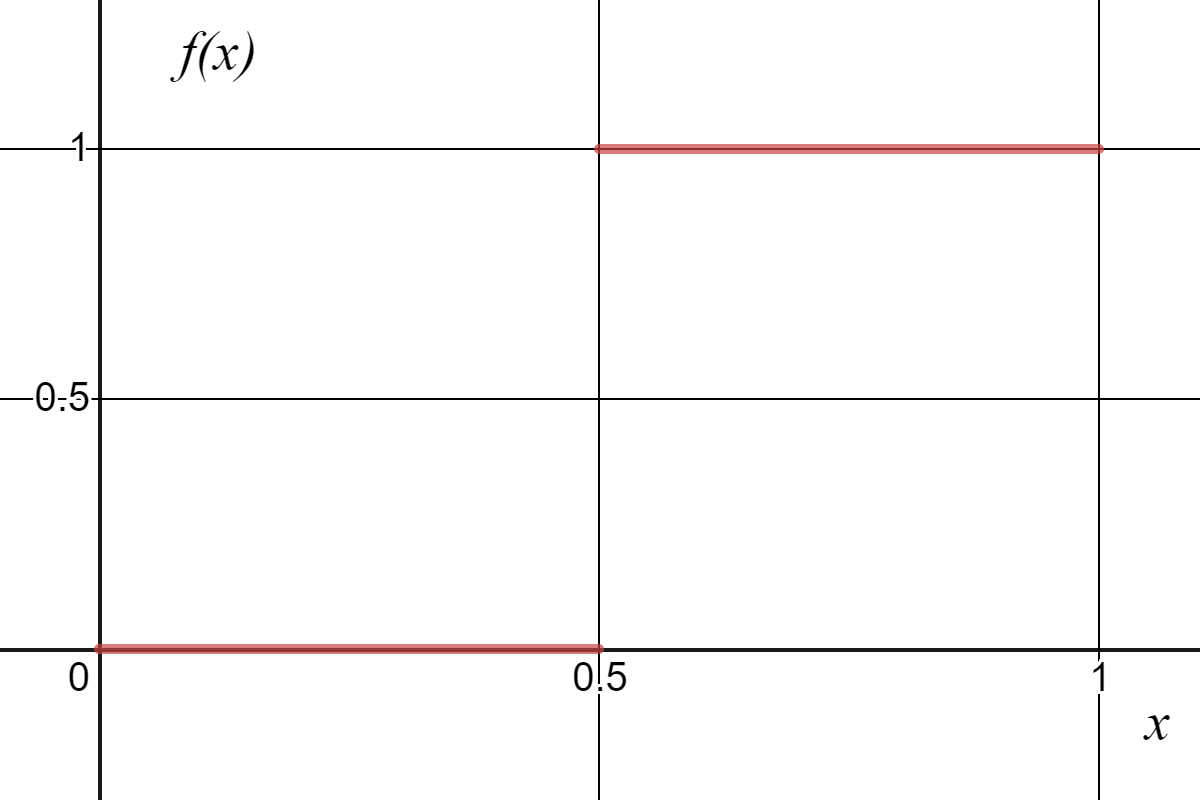
\includegraphics[width=.6\textwidth]{f_function.png}
			\caption{A plot of $f(x)$ in red.}
		\end{figure}
	\end{solution}

\begin{solution}{}{prob13}
		Determine the values for $a_0$, $a_n^e$, and $a_n^o$.
		\tcblower
		We can compute the coefficients $a_0$, $a_n^e$, and $a_n^o$ by projecting onto the functions using the given integral. That is, we will have
		\begin{align*}
			a_0 &= \frac{2}{L}\int_0^L f(x) dx\\
			a_n^e &= \frac{2}{L} \int_0^L f(x) \cos\left(\frac{2n\pi x}{L}\right)dx\\
			a_n^o&= \frac{2}{L}\int_0^L f(x) \sin\left(\frac{2n\pi x}{L}\right).
		\end{align*}
		First, we get
		\begin{align*}
		a_0 &= \frac{2}{L} \int_0^L f(x)dx \\
		&= \frac{2}{L} \int_0^{L/2} f(x)dx + \frac{2}{L}\int_{L/2}^L f(x)dx\\
		&= \frac{2}{L}\int_{L/2}^L dx\\
		&= 1.
		\end{align*}
		Note how we split the integral in order to work with the piecewise function $f(x)$.  Similarly, we will have
		\[
		a_n^e = \frac{2}{L} \int_{L/2}^L \cos\left(\frac{2n\pi x}{L}\right)dx = \frac{\sin(2\pi n)-\sin(\pi n)}{\pi n},
		\]
		which turns out to be zero for every $n$. Lastly, we have
		\[
		a_n^o = \frac{2}{L} \int_{L/2}^L \sin\left(\frac{2n\pi x}{L}\right)dx = \frac{\cos(\pi n)-\cos(2\pi n)}{\pi n}.
		\]
		Thus, we can write 
		\[
		f(x)=\frac{1}{2} + \sum_{n=1}^\infty \frac{\cos(\pi n)-\cos(2\pi n)}{\pi n}\sin\left(\frac{2n \pi x}{L}\right),
		\]
		as the Fourier series for $f(x)$.
	\end{solution}

\begin{solution}{}{prob14}
		Approximate the function $f(x)$ by truncating the sum at:
		\begin{itemize}
			\item $N=0$;
			\item $N=1$;
			\item $N=3$;
			\item $N=10$;
			\item $N=50$;
			\item $N=100$.
		\end{itemize}
		\tcblower
		Now, we can approximate our function $f(x)$ by truncating the above series. That is, 
		\[
		f(x)\approx \frac{1}{2} + \sum_{n=1}^N \frac{\cos(\pi n)-\cos(2\pi n)}{\pi n}\sin\left(\frac{2n \pi x}{L}\right),
		\]
		for some finite integer $N$. We will plot this for the given values.
\begin{figure}[H]
	\centering
	\begin{subfigure}[h]{0.3\textwidth}
		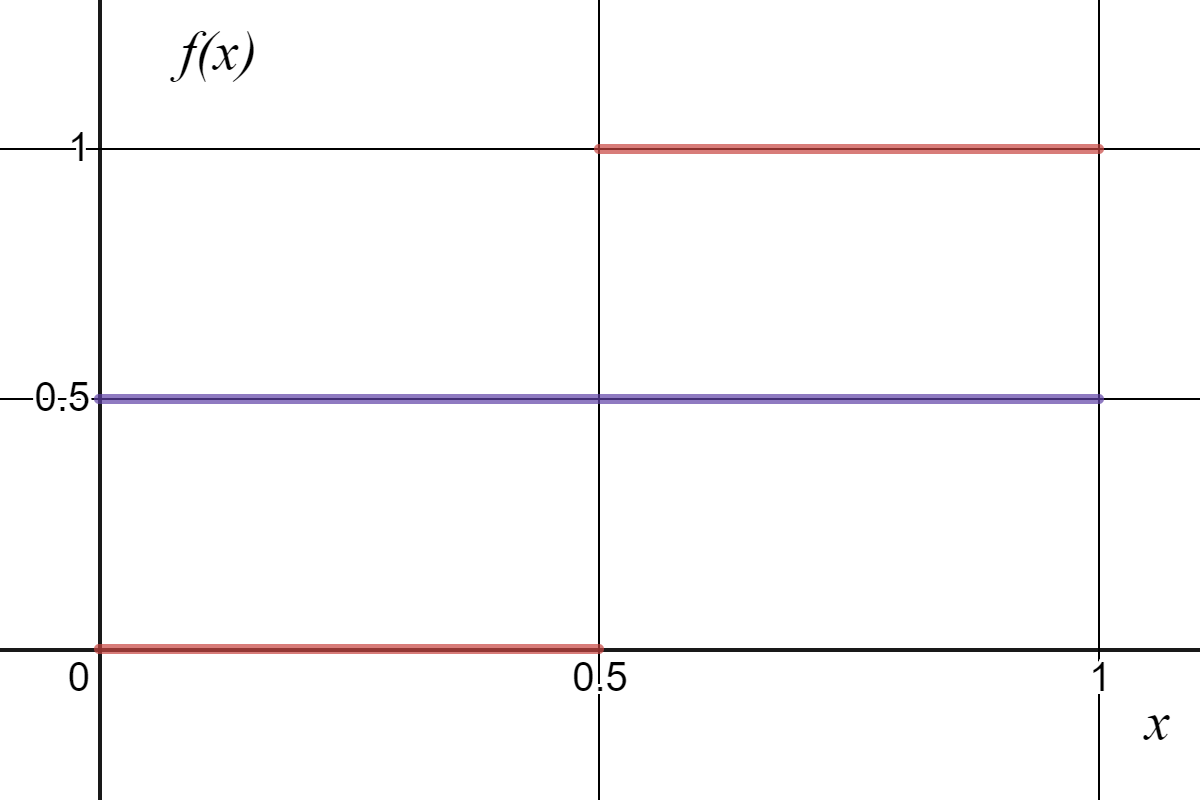
\includegraphics[width=\textwidth]{N=0.png}
		\caption{$N=0$ approximation.}
	\end{subfigure}
	~ 
	\begin{subfigure}[h]{0.3\textwidth}
		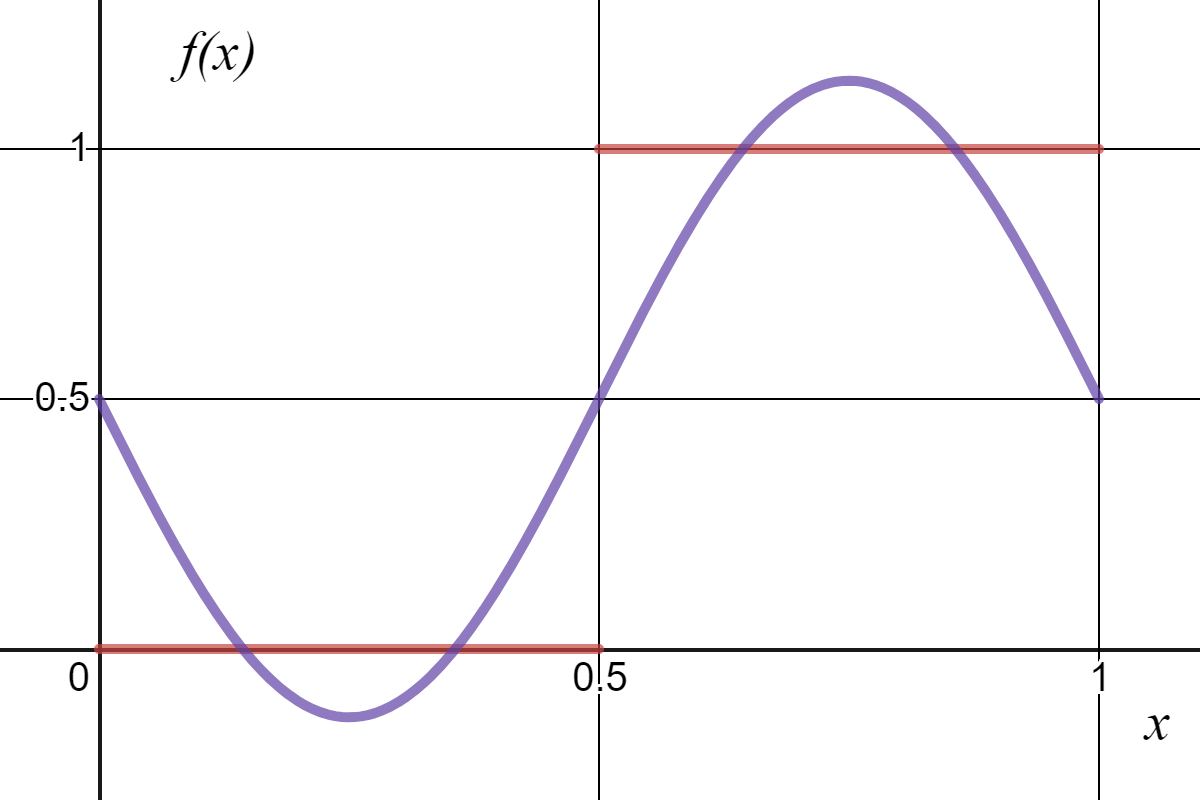
\includegraphics[width=\textwidth]{N=1.png}
		\caption{$N=1$ approximation.}
	\end{subfigure}
	~
	\begin{subfigure}[h]{0.3\textwidth}
		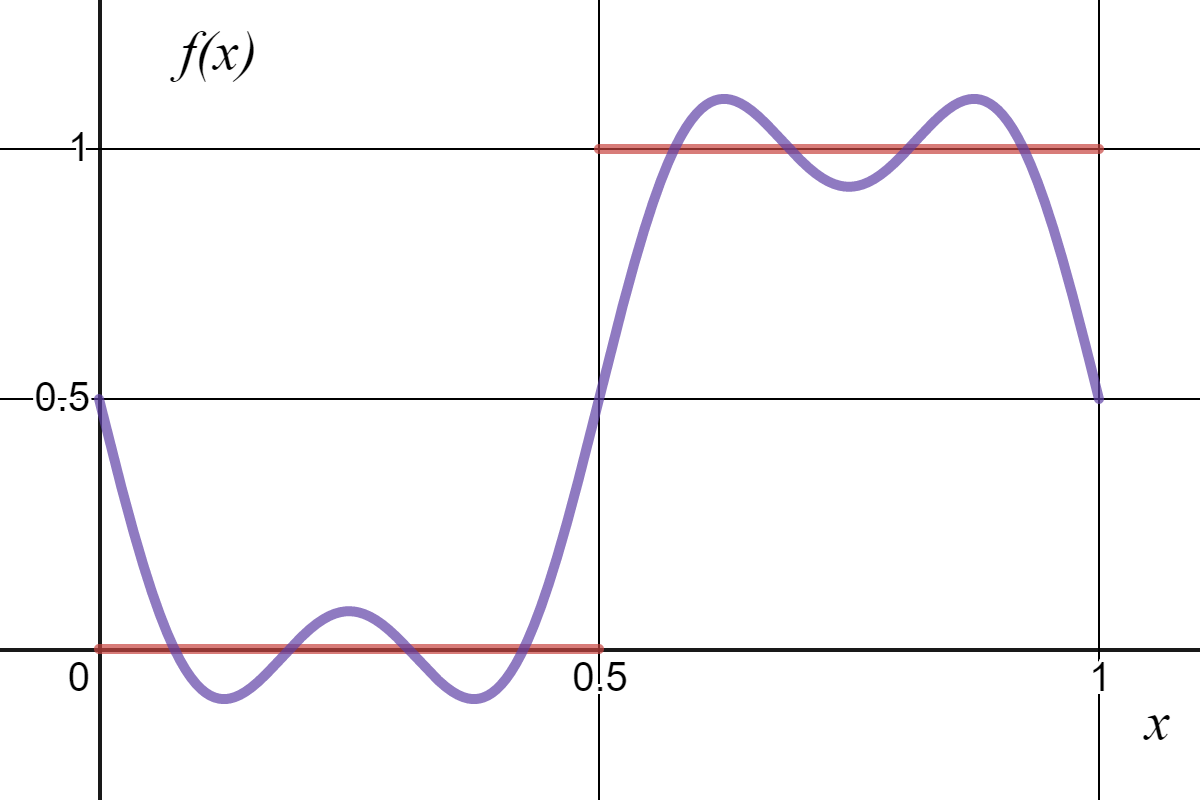
\includegraphics[width=\textwidth]{N=3.png}
		\caption{$N=3$ approximation.}
	\end{subfigure}\\
	
	\begin{subfigure}[h]{0.3\textwidth}
		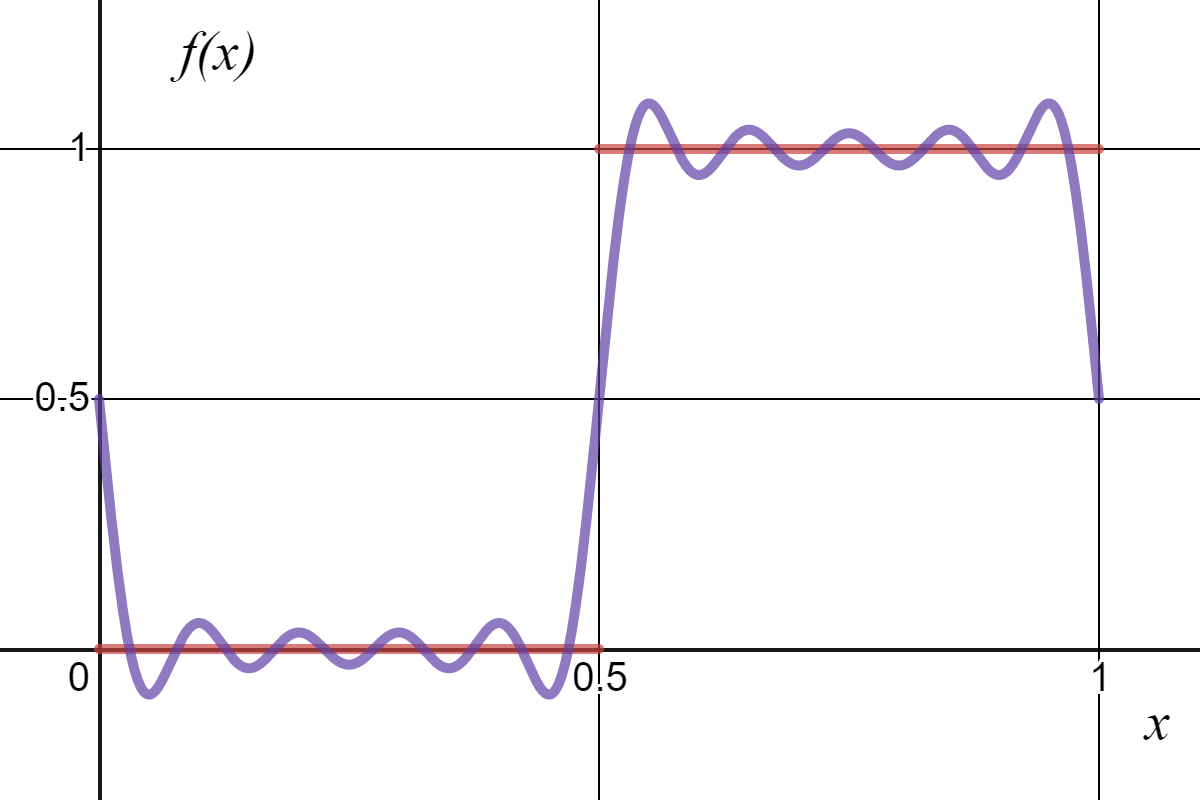
\includegraphics[width=\textwidth]{N=10.png}
		\caption{$N=10$ approximation.}
	\end{subfigure}
	~ 
	\begin{subfigure}[h]{0.3\textwidth}
		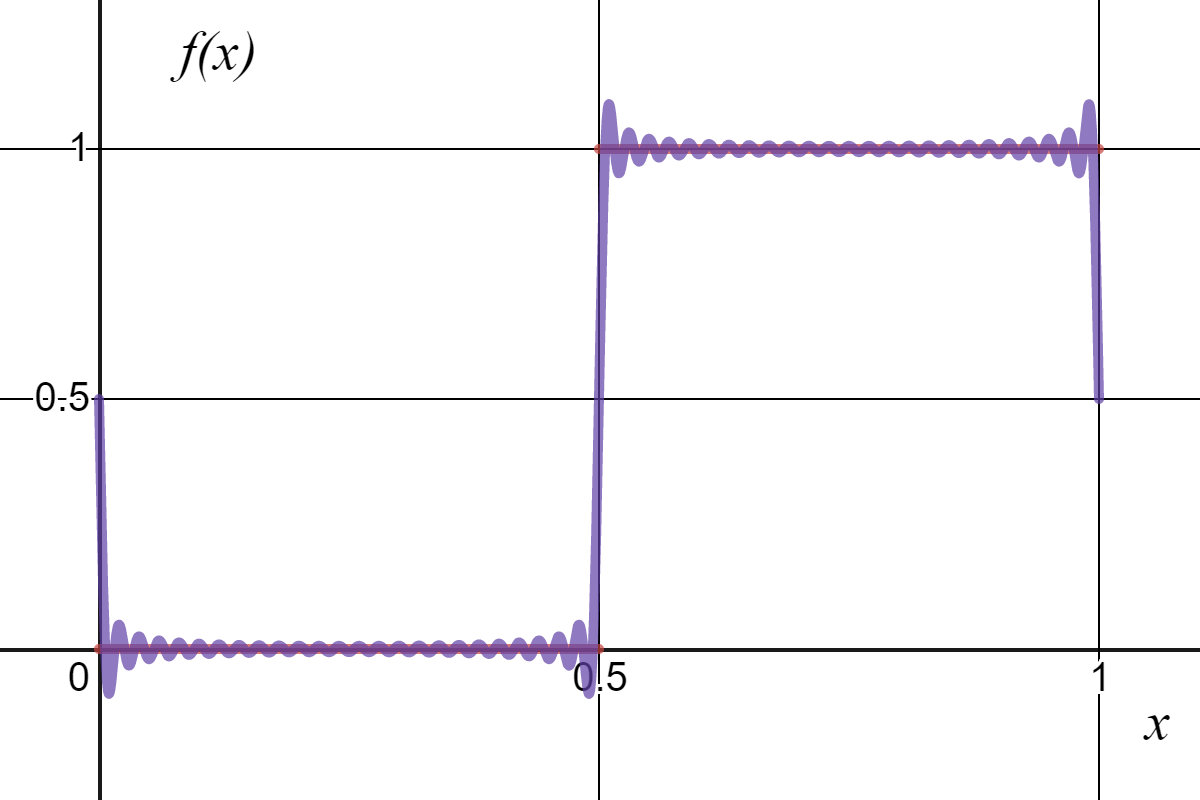
\includegraphics[width=\textwidth]{N=50.png}
		\caption{$N=50$ approximation.}
	\end{subfigure}
	~
	\begin{subfigure}[h]{0.3\textwidth}
		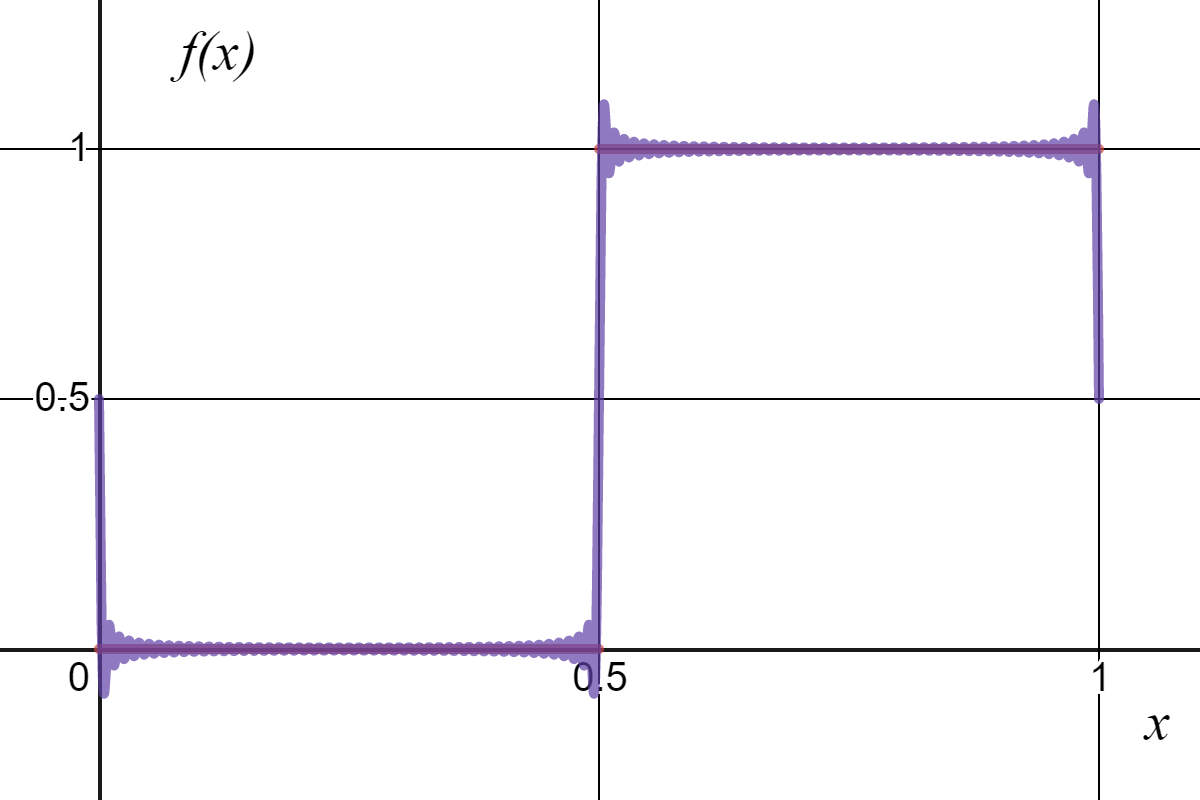
\includegraphics[width=\textwidth]{N=100.png}
		\caption{$N=100$ approximation.}
	\end{subfigure}
\caption{True $f(x)$ in red. Approximations in purple.}
\end{figure}
We can see that the approximation to the function $f(x)$ is done at a fairly low order. A fairly reasonable approximation would be $N=10$ and at $N=100$, this shown to be even better.  Note that if we tried to form a Taylor series for $f(x)$, we would not be successful since the function is piecewise constant.  Thus, for some functions, other forms of series representations prove to be much more powerful.
	\end{solution}

\begin{solution}{}{prob15}
		Write a short paragraph or two on the techniques of spectroscopy and include how the Fourier transform (a slight generalization of the Fourier series) is used. Don't worry about too much detail, just try to learn something new for yourself here! Spectroscopy is an important tool for chemists!
		\tcblower
		One may perform Fourier transform spectroscopy on emitted light in the following way. Say for example, we take a white light (broad spectrum) source and record the emitted light. This emitted light will is truly a combination (superposition) of many different frequencies of light all at once which combine to give a white color.  However, what frequencies of light are being combined in order to have the resulting white light? We can answer this question by taking a Fourier transform of the signal we recieved earlier. Similarly, in Fourier Transform Infrared spectroscopy (FTIR spectroscopy), one tries to measure the absorption of infrared light of different substances in order to determine more about a substance.
		
		Both of these processes are done in the same way.  We measure the intensity of the light over a range of different wavelengths by interfering the broad spectrum light with known wavelengths. This will give us an intensity output at a given frequency, which is exactly the Fourier transform of the broad spectrum light at that frequency.  Once we have interfered the white light at many different values, an approximation of the Fourier transform has been computed and hence we know the frequency components of the light.
		
		In other words, we can often easily measure the coefficients $a_0$, $a_n^e$, and $a_n^o$ for a given function $f(x)$ which is acting as our broad spectrum source.  The interference we perform essentially performs the projection integrals we wrote earlier which allows us to determine the coefficients.  We can picture the function $f(x)$ we had earlier as emitting a continuum broad band of light of wavelengths $L/2$ to $L$. What we would measure is the coefficients we found, which would give us the breakdown of that light into the frequency components. This may seem rather useless as we know $f(x)$. But, in reality, you will measure $f(x)$ via this process and only be able to reconstruct the approximation!
	\end{solution}

\end{document}
